\RequirePackage{snapshot}
\documentclass [10pt, twoside] {article}
\usepackage{float, graphicx, caption, amssymb, natbib}
\usepackage[usenames,dvipsnames]{color}
\usepackage{tabulary}
\usepackage [left=2.5cm, top=2.5cm, bottom=2.5cm, right=3cm] {geometry}  %% see geometry.pdf on how to lay out the page. There's lots.
\geometry{a4paper} %% or letter or a5paper or ... etc
\usepackage{fancyhdr}
\usepackage{xcolor}
\usepackage[scaled]{helvet}
\usepackage{amsmath}
\usepackage{url}
%\usepackage{draftwatermark}
\renewcommand*\familydefault{\sfdefault} %% Only if the base font of the document is to be sans serif

%\usepackage[left]{lineno}
\usepackage[yyyymmdd,hhmmss]{datetime}

%\renewcommand{\linenumberfont}{\normalfont\tiny\color{gray}}
\newcommand{\version}{{v1.0}}

\pagestyle{fancy}
\fancyhead{}
\fancyfoot{}

\fancyhead[L]{\textbf{DefiPlaza white paper}}
\fancyhead[R]{\version}
\fancyfoot[RO,LE]{Page \thepage}

\usepackage{blindtext}

\newcounter {note}
\stepcounter{note}

\renewcommand{\abstractname}{Abstract}

\newcommand {\Note} [1] {
    \marginpar {
        \tiny {
            {\color{gray}{\thenote  \  #1}}
            }
        }
    \stepcounter {note}
}

\newcommand {\MNote} [1] {
    \marginpar {
        \tiny {
            {\color{gray}{#1 }}
            }
        }
}


\begin{document}
\title{Keep CALM and carry on: sustainable DeFi on Radix}

\author {\version { }- Jazzer9F}

\date{\today}

\maketitle

\begin{abstract}
Impermanent Loss is the scourge of liquidity providers in decentralized finance. To make decentralized finance a sustainable solution impermanent loss needs to be dealt with. In this white paper, we present the Concentration-Asymmetric Liquidity Model (CALM) which is specifically designed to make providing liquidity sustainably profitable. The main innovation is that CALM treats trades that increase impermanent loss differently from those that reduce it, thereby reducing the negative impact of impermanent loss. The result is an algorithm which is efficient to implement, has fungible liquidity tokens, allows liquidity concentration, allows true single-sided liquidity add, uses an internal price oracle, creates a bid-ask spread in times of high volatility and (most importantly) vastly outperforms traditional methods in terms of bottom-line performance for liquidity providers.
\end{abstract}

%\linenumbers

\section{Introduction}
In Decentralized Finance the search for high returns inevitably goes hand in hand with soaring risks. A fundamental obstacle is the strong appeal of towering Annual Percentage Yields (APY), a measure that all too often disregards the imminent threats associated with Impermanent Loss (IL). Dissecting historic returns provides a sobering realization: Impermanent Loss often eclipses the appealing APY, resulting in considerable losses for the majority of liquidity providers. Some protocols choose to offer incentives to provide liquidity despite the risks, further complicating net loss making liquidity schemes.

Losses by Liquidity Providers (LPs) are not limited to those protocols refered to as 'degen' protocols in the community. Even some of the most established and well respected protocols leave plenty room for improvement when it comes to impermanent loss. A quant trader going by the name of Alex on X (then Twitter) observed that IL due to toxic orderflow (ie arbitrage) experienced by Uniswap liquidity providers has outweighed their fee income at the largest liquidity pair on Uniswap v3 (ETH/USDC) by just over 100 M\$ \cite{alex, dune}. That is one hundred million dollars lost to the arbitrageurs at just one single liquidity pair! Shockingly, the concentrated liquidity feature caused Uniswap LPs to be on average worse off \emph{after fees} than Uniswap v2 features would have been \emph{before fees}. A study published by Bancor investigated 17 large pools in just the first half year of Uniswap V3 lost a collective 60.8 M\$ \cite{bancorIL}. Why would any rational actor supply concentrated liquidity under those conditions?

The low interest environment of the early 2020s has caused capital to chase yield in irresponsible ways, and DeFi was one of the routes where yields were seemingly outperforming those in the traditional financial system. For a short while, the meteoric rise of decentralized exchanges such as Uniswap seemed obvious and inevitable, but the cold hard truth revealed by Alex's analysis is that the basic constant product AMM with concentrated liquidity (ie Uniswap v3) simply do not provide a sustainable operating model. The dream of passively providing liquidity and generating a net income appeared to remain just over the horizon.

Any DeFi ecosystem can only be viable in the long term if the products are beneficial to all participants. The ever present threat of impermanent loss, especially for concentrated liquidity positions, has proven to be a significant barrier to long term viability. In this paper, we propose a novel algorithm that aims to mitigate the risk of impermanent loss. It is key to understand that impermanent loss can never be prevented completely, as the only way to prevent it from happening is to not trade away from equilibrium which is the same as to say that we would never trade at all. Thus, if we want to provide our tokens to a liquidity protocol so as to create an opportunity to earn fees, we need to expose ourselves to the risk of impermanent loss to a certain degree. However, by applying the CALM model introduced in this paper, the risk of long term impermanent loss may be greatly reduced when compared to a traditional liquidity protocols.

\subsection{Context and prior art}
One of the first proposals for a liquidity protocol was the Bancor Network \cite{bancorToken, bancorWP}, pioneering the space in 2017 and continuously innovating to this day. During DeFi summer (2020 until early 2021), many innovative DeFi products were released. Decentralized exchanges were truly popularized with the rise of Uniswap \cite{uniV1, uniV2, uniV3}, with their V2 constant product liquidity pools being the first to reach into the billions of dollars in total value locked (TVL). Curve revolutionized capital efficiency for liquidity pools holding tokens of correlated value, such as stable coins \cite{curve, curveV2}. Balancer introduced imbalanced pools \cite{balancer}, and Dodo introduced the predictive market maker (PMM) \cite{dodo}, which we'll get back to in section \ref{subsubDodo}.

The flurry of innovation combined with the high availability of capital lead to extreme growth, to the point that the Ethereum network became so congested that transaction fees reached levels that simply made in impossible to use for day to day applications. It was during this time that DefiPlaza was born, creating a DEX with high capital efficiency and the lowest possible gas costs per transaction. DefiPlaza uses a multitoken variant of the constant product market maker that Uniswap popularized for token pairs. It works well, and remains to this day the cheapest way to execute token swaps on Ethereum.

DefiPlaza on Ethereum \cite{defiplaza1, defiplaza2} was inspired by Balancer. For DefiPlaza on Radix, the objective became to develop an IL mitigating algorithm. For that, our research suggested the Dodo liquidity protocol gave a better starting point. Thus, we need to introduce Dodo before introducing the CALM model.

\subsection{Dodo -- A different way of looking at liquidity} \label{subsubDodo}
Dodo stands out in the crypto space, thanks to its innovative Predictive Market Maker (PMM).Unlike other decentralized exchanges (DEXes), Dodo separates liquidity provided by its liquidity providers (LPs) into separate pools: Base Liquidity and Quote Liquidity. In addition, Dodo employs a meticulous record-keeping process for each liquidity pool type, continuously monitoring which token is in shortage relative to its target. Furthermore, Dodo leverages a flexible parameter "$k$", which fine-tunes the concentration level of the liquidity. A $k$ value of 1 mirrors the constant product autonomous market maker (AMM), mathematically equivalent to Uniswap V2, whereas a $k$ value of 0 signifies maximum liquidity concentration, yielding a constant sum AMM with no price impact. Note that although the Dodo smart contracts don't allow for it, there is no fundamental barrier to use values of $k$ larger than one, implying sparser liquidity than the default constant product AMM. In this paper, we will consider $k$ values larger than zero, including those larger than one.

Without loss of generality, from here on out we will assume that base token is in shortage when discussing calculation examples. In the case of base shortage the Dodo liquidity protocol is governed by the following equations:

\begin{align}
p_{\text{margin}} & = \left( (1-k) + k\left(\frac{B_0}{B}\right)^2 \right) p_0 \label{eq:price} \\
\Delta Q & = \left( B_{0} - B \right) \left( (1-k) + k\frac{B_{0}}{B} \right) p_{0} \label{eq:curve}
\end{align}

Equation \ref{eq:price} gives the spot price at any given time, which depends solely on the reference price $p_0$ and the ratio between the target for the base tokens $B_0$ and the actual amount of base tokens $B$. This ratio is always greater than one since the base tokens are in shortage. Equation \ref{eq:curve} is the result of integrating the price curve from equilibrium to a given base token shortage to give the amount of quote tokens $\Delta Q$ held in excess of the quote token target $Q_0$. This is the amount of quote tokens the pair has taken in while moving the base token amount from $B_0$ to $B$.

The key insight that enabled the CALM model described in the next chapter is that due to separating the liquidity pools for base and quote, and managing shortage with respect to the target token amount, the Dodo implementation allows us to identify which trades increase IL (ie those that increase an existing shortage) versus those that reduce IL (ie those that move towards equilibrium). There is nothing stopping us from applying different bonding curves, as long as we are careful not to create or destroy value at the interface. Treating trades increasing/reducing IL differently is exactly the core idea behind CALM.

As a side note, the reference price $p_0$ in Dodo is supplied by an external price oracle, which is where the 'predicitve' part in the PMM name comes from. The external oracle part of the Dodo protocol is explicitly not followed in our protocol. In CALM, the reference price is tracked by an internal price oracle for which the oracle inspiration was the internal oracle mechanism of Curve v2, although the mechanism for reference price update in CALM is vastly different from that in Curve. 

\section{Concentration-Asymmetric Liquidity Model (CALM)}
The CALM model used at DefiPlaza applies different levels of liquidity concentration when increasing IL ($k_{out}$) versus when reducing IL ($k_{in}$). Specifically, the liquidity concentration is always sparser when increasing IL than when a trade reduces IL (ie: $k_{out} > k_{in}$). Intuitively, trading along a sparser bonding curve means that to get to a certain shortage of base tokens, you need to supply more quote tokens than if the liquidity concentration is higher. Thus, if we apply this mechanism, a trade away from equilibrium creates a higher $\Delta Q$ than was expected at the same shortage point along the curve trading back towards equilibrium. When mapping back to the IL reducing curve, these 'additional' tokens can be used to either increase the reference price $p_0$ or increase the base target amount $B_0$.

\subsection{Increasing IL -- trading away from equilibrium}
When trading away from equilibrium, we use $k_{out}$ as concentration parameter, and solve equation \ref{eq:curve} for $B$. Rearranging and using the helper variables of shortage ($\Delta B = B_0 - B$) and scaled surplus ($\Delta Q' = \Delta Q / p_0$) we get an equation that is quadratic in $\Delta B$, hence solving it gives two solutions. Only one of these has physical meaning, so the other one is discarded. The solution we're looking for is given by equation \ref{eq:baseSolution} below:

\begin{align} \label{eq:baseSolution}
	\Delta B &= \frac{B_0 + \Delta Q' - \sqrt{B_0^2 + \left(4k_{out}-2\right)B_0 \Delta Q' + \Delta Q'^2}}{2\left(1-k_{out}\right)}
\end{align}

The $\Delta B$ gives the total base token shortage with respect to equilibrium. To compute the amount of output tokens for any trade, we can use equation \ref{eq:baseSolution} filling in the new surplus value and simply subtracting the original shortage. Note that equation \ref{eq:baseSolution} suffers from division by zero when $k_{out}$ is equal to one, as both the numerator and the denominator tend to zero. When $k_{out}$ is exactly equal to one, equation \ref{eq:curve} may be simplified before solving for $\Delta B$. For this special case we can use the simplified equation \ref{eq:special} to calculate the shortage before and after the trade.

\begin{equation} \label{eq:special}
\Delta B = \frac{B_0 \Delta Q'}{B_0 + \Delta Q'}
\end{equation}

\subsection{Reducing IL -- trading towards equilibrium}
Still assuming a base shortage in the pair, we use $k_{in}$ as concentration parameter for trades towards equilibrium, ie trades which give base tokens as input and quote tokens as output. Using the helper variable $\Delta B = B_0 - B$, and setting $k = k_{in}$ in equation \ref{eq:curve} yields equation \ref{eq:quoteSolution} after some rearranging.

\begin{align} \label{eq:quoteSolution}
	\Delta Q  &= \frac{\Delta B \left(B + k_{in} \Delta B \right)}{B} p_0
\end{align}

This equation describes the curve over which the trades are executed. We can calculate the amount of output quote tokens for an input amount of base tokens by solving equation \ref{eq:quoteSolution} for the corresponding values of $B$ and $\Delta B$.

\subsection{Emerging bid-ask spread and reference filter}
When trading away from equilibrium along the sparser curve, the shortage doesn't increase as much as it would have for the denser curve to reach the same spot price. This means that if we don't change any other values such as the reference price and/or the target values, the inward curve and the outward bonding curves will have a different spot price. The spot price of the inward curve is the bid-price, while the spot price for the outward curve is the ask-price for the base token. Thus, when trading far away from equilibrium, a bid-ask spread spontaneously arises. When there is sufficient volatility in the market, this bid-ask spread may be crossed generating additional income for the liquidity providers. The size of the spread depends on the ratio between $k_{out}$ and $k_{in}$, with a greater ratio causing a larger spread.

Having a bid-ask spread can be favorable during times of volatility, but when the market is quiet we prefer to close this price gap to increase volume. There are several ways to close the spread. One could raise the reference price and/or lower the target amount, shifting the bid price towards the ask price. Alternatively, one could change the reference price for the outward trades to move the ask price closer to the bid price. One could also manipulate the level of concentration but that approach out of scope for the CALM model.

In DefiPlaza, the bid-ask spread is closed from both sides. Both the bid and ask prices are moved towards each other by manipulating their respective reference prices. There is room to increase the reference price for the inward curve due to the excess quote tokens earned by trading outward on a sparser liquidity curve. Whatever gap remains is closed by reducing the reference price on the outward trading curve.

The bid-ask spread is closed gradually over time (using an exponential filter), such that in times of high market volatility the LP providers actually profit from the additional income generated as the market crosses the bid-ask spread. As far as we know, this feature is unique to DefiPlaza. During times of high market volatility LPs at other DEXes only pocket the fees the trades flowing back and forth. With the CALM model, the LPs actually benefit from the different pricing on the inward/outward curves which is the main driver of the improved performance demonstrated in section \ref{sec:results}.

\subsection{Moving back and forth between the trading curves}
Starting from equilibrium, if one or several trades increasing IL have occurred, trading in the other direction requires using the other bonding curve. This needs to be done carefully so as to ensure that the curves are respected without creating opportunity for exploitation.

Specifically, moving from trading with $k_{out}$ to trading with $k_{in}$ we have an excess of $\Delta Q$ to fit equation \ref{eq:curve} with the same $p_0$ and $B_0$ values. To make the reserves fit the trading curve, we can either increase $p_0$, increase $B_0$, or a combination of both. In CALM, we initially allocate the excess tokens to a higher $B0$ but over time gradually shift to an adjustment of $p0$ instead. Thus, if the price reverts relatively quickly, the liquidity providers will end up with a higher amount of base tokens. However, if the price stays elevated, the reference price will be adjusted and the target amount is reverted to the original value. Depending on how much time has passed, the actual value for $p0$ used for new trades is calculated using a filter. From that $p0$ value, we calculate the corresponding base target $B_0$ by solving \ref{eq:curve} for $B_0/B$ and multiplying the result by $B$. Equation \ref{eq:curve} is quadratic in $B_0/B$ and we again find two solutions out of which only one has physical meaning. When we set $\Delta Q'=\Delta Q / p_0$, the desired solution is given by \ref{eq:target}:

\begin{equation} \label{eq:target}
	\frac{B_0}{B}_{temp} = \frac{2 k_{\text{in}} + \sqrt{1 + 4 k_{\text{in}} \Delta Q' / B} - 1}{2 k_{\text{in}}}
\end{equation}

Equation \ref{eq:target} is only valid for values of $k_{in}$ larger than zero, which are the only cases that we are interested in here. The temporary target value calculated by this equation is used for any trades reducing IL. After a trade is completed, the permanent target value needs to be updated to fit the curve for the steady state value of $p_0$ computed earlier.

Symmetrically, if we move from trading in the direction reducing IL to the direction increasing the shortage and hence the IL, we also need to recalibrate the curve. Above, the recalibration happened based on equation \ref{eq:curve}. Here, we recalibrate based on spot price (equation \ref{eq:price}). For the outward trade direction, we match up the spot price with the steady state spot price for the inward curve. To do the alignment for a given shortage, we need to temporarily change the reference price $p_0$ for any outgoing trade. The value used is given by equation \ref{eq:refprice} which is found by solving equation \ref{eq:price} for $p_0$:

\begin{equation} \label{eq:refprice}
	p_{0_{temp}} = \frac{p_{spot}}{(1-k) + k\left(\frac{B_0}{B}\right)^2}
\end{equation}

Using these temporary values when moving back and forth between the curves guarantees continuity of trading while always making adjustments to the benefit of the liquidity providers. 

\subsection{Adding liquidity}
As discussed before, liquidity is tracked for each side of the reference price separately rather than lumping all tokens together like most protocols. The amount of liquidity on each side of the pair need not be equal, and it's entirely possible that there is a difference in ROI between the two sides. In keeping with the sustainable DeFi principle, the objective is to make liquidity provision sustainably profitable for each side, or at least to significantly reduce the risk of incurring a loss. Ideally, the pair stays mostly in balance and each side of $p0$ contains mostly one type of token. The pool for the token that is in shortage at any given time does contain some amount of the other token ($\Delta Q$ in the examples given). However, adding liquidity is always a a single token affair.

When adding liquidity, the CALM pair checks whether the token that is being added is in shortage. If there is no shortage, the liquidity provider is simply granted LP tokens in ratio to how much liquidity is added with respect to how much was already present. If the token \emph{is} in shortage the trading curve is recalibrated to the new position, and the liquidity provider is granted LP tokens in ratio to the increase of the target value resulting from the reduced shortage.

\subsection{Differences with respect to Dodo / Curve}
DefiPlaza builds on the Dodo approach to liquidity pools, which in itself builds on the Uniswap model. Furthermore, some features around the reference price are inspired by Curve. The differences between CALM and Dodo are listed below, with reference to Curve where relevant.

\begin{enumerate}
\item The asymmetric liquidity model gives rise to a natural bid-ask spread. This allows LPs to profit from rapid price swings with more income than just the fees of the for- and backward trades. The size of the bid-ask spread can be configured by the ratio of concentration for IL generating/reducing trades, with the spread closing completely over a configurable time period. When prices are stable, the spread will be small whereas when there are rapid price changes the spread will be (temporarily) large.
\item The Dodo implementation is focused on liquidity concentration, even though the math also allows de-concentration with respect to the constant product AMM. The CALM model uses de-concentration, which results in reduction of impermanent loss risk at the cost of lower fraction of tokens traded and correspondingly lower fee income. Analysis in section \ref{sec:results} ahead will show that the impact of impermanent loss protection outweighs the reduced fee income.
\item CALM utilizes an internal price oracle - a feature inspired by Curve's v2 liquidity pool model so as to do away with the need for an external oracle. Dodo uses an external price oracle. Doing away with the external price signal yields a significant improvement to safety as oracle pricing is a common point of failure and/or attacks in DeFi.
\item Increasing the oracle price of a token when that token is in shortage essentially incurs a loss to the liquidity providers. In Dodo, the price is always updated when the external oracle price updates. In Curve, the price is only updated when the fee income is more than twice the cost to update the price. In CALM, the oracle price update happens gradually over time and only to to extent that can be afforded from the excess tokens from the asymmetric liquidity mechanism.
\item When adding liquidity to a token that is in shortage, a Dodo liquidity provider incurs an immediate loss, with the beneficiaries being the existing LP providers. There effectively is a fee to add liquidity, which gets higher and higher the more the pool is imbalanced and which disincentives adding liquidity when it is needed the most. In CALM, the fair amount of LP tokens is calculated such that there is no gain/penalty to the new liquidity provider versus exisiting LPs.
\end{enumerate}

\section{Results} \label{sec:results}
As a test, the CALM algorithm was run against two specific historic datasets. First, there is the historic data for ETH/USD which is the same pair that Alex initially identified as hugely problematic for Uniswap v3 liquidity providers. Secondly, we take BTC/ETH as the prototypical crypto-to-crypto trading pair. For this pair we assume the price movement is somewhat muted as both of the tokens in the pair are impacted by much of the same macro factors.

The datasets are exchange price data sampled at 1h intervals, freely available on the internet \cite{data}. Trades are executed against the close price at each hour mark, if the price differential between the exchange and the DefiPlaza pair is large enough. We assume a 0.3\% margin is required for arbitrageurs to cover their costs and execute a trade. We model only this 100\% toxic order flow to get a conservative estimate of fee income. The Uniswap portfolio is simulated under the same conditions, to ensure the 0.3\% trading fee is also taken into account.

\begin{figure}[!htbp]
\centering
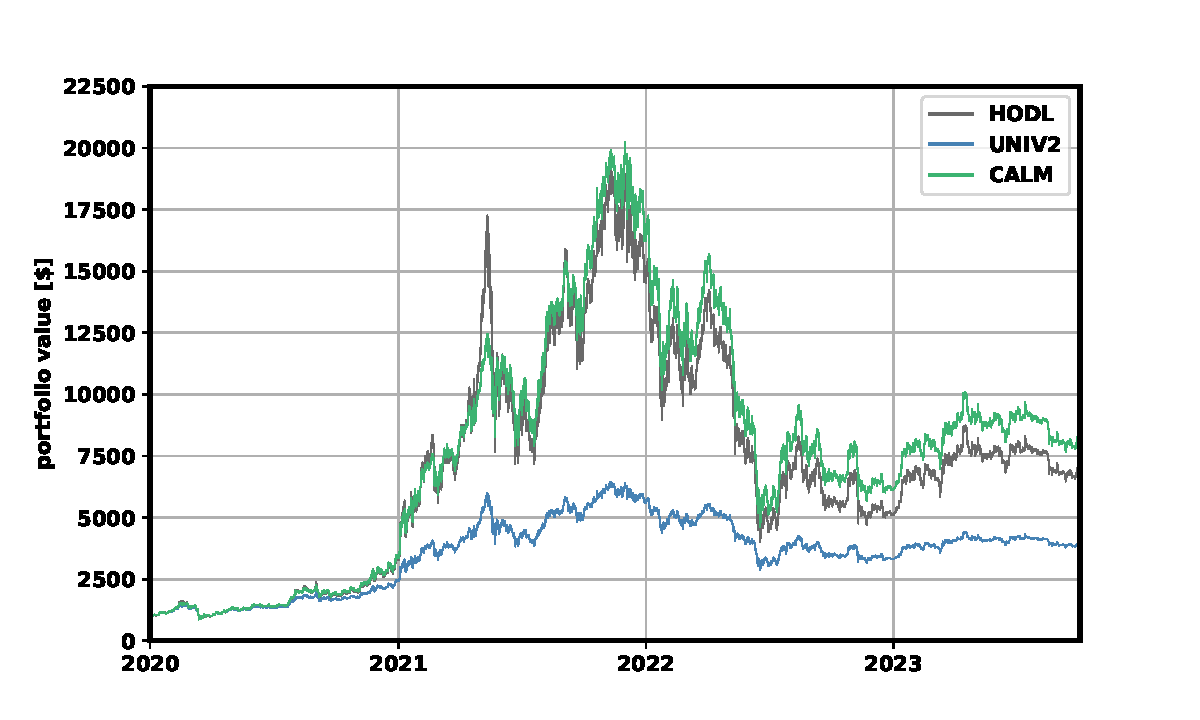
\includegraphics[width=\textwidth,keepaspectratio]{figures/ETH_USD.pdf}
\caption{Superior performance of CALM with respect to classic Uniswap v2 style AMM for ETH/USDC pair under heavy price volatility.}
\label{fig:resultgraph}
\end{figure}

Figure \ref{fig:resultgraph} shows the performance of 1000\$ invested in a Uniswap v2 pair (ie 500\$ in USDC and 500\$ worth of ETH) on January 1st 2020 (when ETH was at \$129) against the simply holding the same portfolio over the same time, versus investing in a CALM pair ($k_{in}=0.15$, $k_{out}=20$, fee at 1\%). Despite an overall ETH price increase of more than 12x, the CALM pair is profitable with respect to the HODL strategy. The Uniswap v2 pair underperforms due to impermanent loss, and we know from Alex's analysis that Uniswap v3 providers do even worse due to concentrated impermanent loss.

It is worth noting that that during the initial extreme runup of May 2021 the CALM strategy fails to follow the HODL value, which demonstrates that if there is strong and persistent one-directional price movement CALM will still accumulate IL, though to a much smaller extent than other liquidity protocols such as the Uniswap V2 pair. By the start of 2022 the CALM pair is clearly in the plus with respect to the HODL strategy, while the Uniswap v2 pair still sits at around 45\% loss after fees.

\begin{figure}[!htbp]
\centering
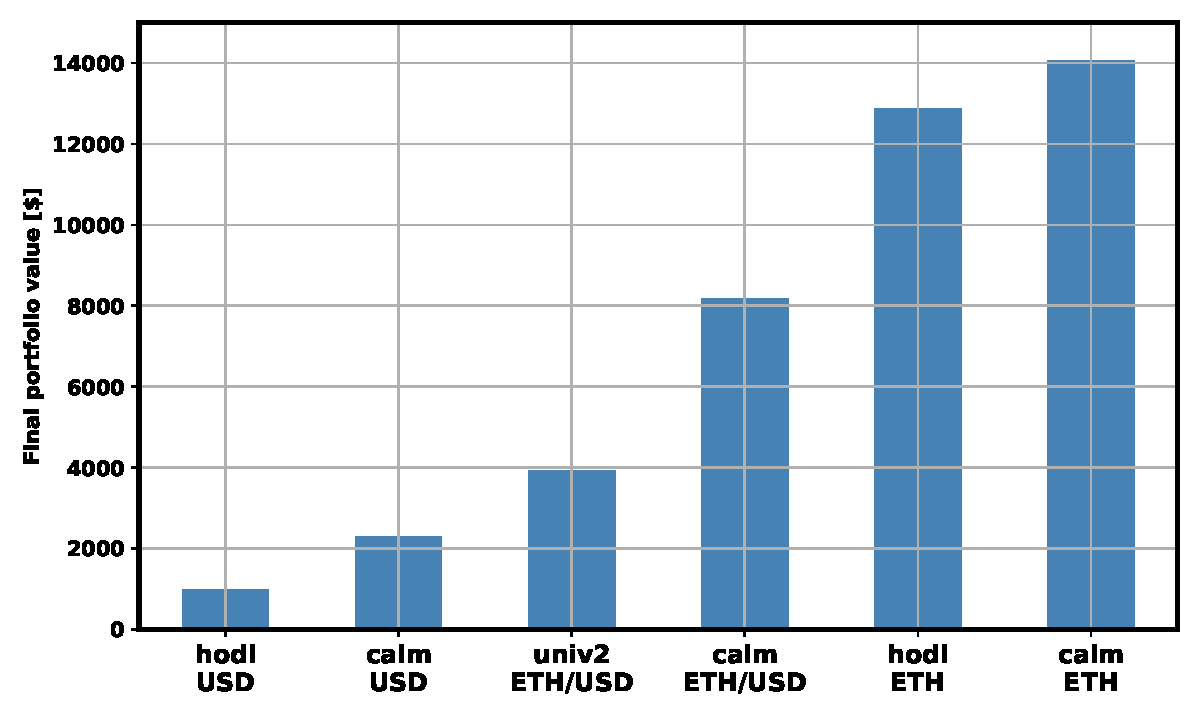
\includegraphics[width=\textwidth,keepaspectratio]{figures/returns.pdf}
\caption{Final returns of various portfolios showing outperformance of the CALM liquidity model.}
\label{fig:returns}
\end{figure}

Figure \ref{fig:returns} shows the final value of various possible portfolios over this period, assuming a 1000\$ starting value for each portfolio. In CALM, you can supply single sided liquidity, and each liquidity type will have it's own ROI. Providing liquidity to CALM outperformed holding the token outright for both USD and ETH. Critically, supplying just ETH results in a higher final value than just holding ETH over the same period despite the 12x price increase of ETH with respect to USD. Supplying USD to CALM over this period results in more than 130\% yield. Supplying ETH to CALM over this period would have resulted in an additional 9.2\% of ETH over just holding it, representing an additional 118\% of yield over the already impressive 1287\% of returns from the price rise of ETH. In summary, CALM clearly beats IL over the Jan-2020 to Sept-2023 period on the ETH/USDC pair under pure toxic order flow.

It is also worth noting that the 1\% fee used in the CALM pair is larger than the 0.3\% fee in the Uniswap v2 pair. However, if we would apply a 1\% fee to the Uniswap v2 pair that doesn't significantly change the results as the accumulated impermanent loss simply dwarfs the fee income for the Uniswap pair. Thus, the vastly improved performance for the CALM pair does not originate from the higher fee, it is mostly due to the IL mitigating properties of CALM.

As a final note, the analysis here was limited to one trade per hour from only toxic order flow. In reality, many trades can happen in an hour and of course there is not only arbitrage order flow but also genuine trading (uninformed flow) that would result in higher fee income. With the 1\% trading fee, it is likely that the CALM pair would get fewer trades from the uninformed order flow than the Uniswap pair would. However, it is our firm belief that the best path towards making money as an LP in DeFi is to stop losing money as an LP in DeFi. Thus, reducing impermanent loss to where it can reliably be expected to be smaller than LP income in the long run is more important than maximizing for trading volume and fee income itself.

\section{Conclusion}
To conclude, we have introduced a ground-breaking algorithm, the Concentration-Asymmetric Liquidity Model, inspired by Dodo and Curve to mitigate impermanent loss risk. A sustainable return is not an illusion, as confirmed through backtesting with pure toxic order flow under appropriate settings. To make DeFi work sustainably a shift in the modus operandi is needed, away from focusing on high APY and trading volumes and towards focus on long term bottom-line performance. Rather than concentrated liquidity, we may need to look at de-concentrated liquidity if we are to defeat the spectre of impermanent loss. At Radix, DefiPlaza will demonstrate that the CALM model together with higher fees may come at lower volumes but will yield higher returns to the liquidity providers than existing protocols. For the first time that we know of, a purely passive liquidity strategy may beat impermanent loss even for trading pairs with different underlying fundamentals.

Furthermore, The CALM model opens up a whole new class of algorithms for future research, where trades increasing impermanent loss are treated differently in some way from those that reduce impermanent loss. Furthermore, our design empowers the ecosystem by accommodating pure single-sided liquidity and concentrated liquidity, both supported by fungible liquidity provider tokens, under one effective execution.

\appendix
\section{Radix -- A quantum leap in UX/devX for DeFi}
One of the reasons for the relatively slow adoption of DeFi in society at large is the user experience. Using dApps is complex and risky. When you sign a transaction, it is an unintelligible string. The same for accounts. Losing your seed phrase means losing your tokens. Hacks and exploits follow each other up in rapid succession. As an end-user, it's just not a great experience. For developers, it's not much different. Building a secure dApp on Ethereum is hard, it's easy to make mistakes even if you are well intentioned.

Enter Radix, which has been built from the ground up with the explicit objective to on-board a billion users onto a single global DeFi ecosystem. The Radix Babylon ledger, released at the end of September 2023 introduces the following features to support that mission:
\begin{itemize}
	\item A scalable platform: The ledger was designed for full state sharding. Even though actual sharding isn't enabled in the Babylon network, the data architecture is built to support it in the next deployment. This makes the ledger future-proof.
	\item The Radix Engine: Tokens and wallets behave as real physical objects, with their logic governed by the Radix Engine. This makes Radix far more intuitive to use, and it becomes much harder to make mistakes both for end-users and developers.
	\item Human readable transactions. When you sign a transaction on the Radix wallet, it shows exactly what will happen in the wallet, giving users insight into what they're signing off on.
\end{itemize}
Another key feature making Radix a great platform to build DeFi applications on is the developer royalty system. The royalty feature enables applying a charge for on-chain transactions on top of the gas fee. Royalties will enable DeFi protocols to recover their operating costs directly from consumers in an elegant manner, without requiring tokenization or adding overhead logic to the smart contracts. Apart from LP profitability, simply covering operating cost is another key enabler for sustainable DeFi that is frequently overlooked.


%\input{01_introduction}

%\input{04_results}
%\input{05_summary}

\bibliographystyle{plain}
\bibliography{references}{}

\end{document}
